In games of imperfect information, the players are not always sure of the current state of the game. That is, one or more players cannot tell apart two or more states of the game. This is a classic application of a possible worlds model. In this section based on \cite{benthem2001a}, we are going to combine game trees and possible worlds models in order to model games of imperfect information.

% { \color{red} I don't think bisimulations are important in this article. This is a introductory article on the connections between game theory and epistemic logic. Bisimulations are a more advanced tool for reducing the size of your games so that they are easier to handle. Hence, they are mostly a tool for gaining efficiency and efficiency is not in introductory topic. I would rather describe how to compute the Nash equilibrium of the Liar's dice example. }

\subsection{Perfect information game trees} \label{seq:perfect-information}

{ \color{red} These is possibly too much theory in this subsection but I wasn't quite sure where this subsection was headed when I started. }

First, we consider two-player games of perfect information: Given a set $ \atomicprops $ of atomic propositions, a game tree $ M = (S, \{ R_{a} : a \in A \}, V) $ for such a game is a set $ S $ of states, a set containing one binary relation $ R_{a} \subseteq (S \times S) $ for each action $ a $ in the set $ A $ of all actions, and a valuation function $ V : S \rightarrow 2^{\atomicprops} $ \cite{benthem2001a}. The actions are also called moves. The states are partitioned among the players, so that each state is controlled by exactly one player. We let $ \atomicprops $ contain the propositions $ \turn_{i} $ and $ \win_{i} $ for each player $ i \in I $ in the set of players $ I $. We define $ V $ such that $ \turn_{i} $ holds of a state $ s $ if and only if player $ i $ controls $ s $. Also, we define $ V $ such that $ \win_{i} $ holds of a state $ s $ if and only if player $ i $ wins at $ s $. Finally, we let $ \leaf $ be true of exactly the leaves of $ M $.

In order to express properties of a state in a game $ M = (S, \{ R_{a} : a \in A \}, V) $, we introduce a modal language with the following syntax, where $ a \in A $ is any action and $ p \in \atomicprops $ is any proposition:
\begin{align*}
\alpha &::= a \barspace \alpha_{1} \cup \alpha_{2} \barspace \alpha_{1} \alpha_{2} \barspace \alpha^{\ast} \\
\beta &::= \langle \alpha \rangle \barspace [\alpha] \barspace \beta_{1} \beta_{2} \\
\gamma &::= \beta p
\end{align*}
Here, $ \alpha $ generates formulas describing sets of sequences of actions. The Kleene star denotes arbitrary finite iteration. The symbol $ \beta $ generates modalities and $ \gamma $ is the starting symbol. The expression $ \langle \alpha \rangle \phi $ denotes that $ \phi $ holds in some state resulting from performing one of the actions of $ \alpha $. The expression $ [\alpha] \phi $ denotes that $ \phi $ holds in all states resulting from performing all actions of $ \alpha $.

A \emph{strategy} $ \sigma : S \rightarrow A $ for player $ i $ is a partial function from a state $ s $ with $ \turn_{i} $ to an action available from $ s $. If every action occurs at most once in the game tree, we can view a strategy as a set of actions. With this view, a \emph{winning strategy} $ \sigma $ for player $ i $ is one satisfying the following \cite{benthem2001a}:
\begin{gather*}
\WIN_{i} \leftrightarrow (\leaf \wedge \win_{i}) \vee (\turn_{i} \wedge \langle A \rangle \WIN_{i}) \vee (\neg \turn_{i} \wedge [A] \WIN_{i}) \\
[A^{\ast}](\turn_{i} \rightarrow \langle \sigma \rangle \WIN_{i})
\end{gather*}
Here, we use the shorthand notation $ A $ for the $ \alpha $-formula $ a_{1} \cup a_{2} \cup \dots $ describing the choice between all possible actions $ a_{1}, a_{2}, \dots $. The first formula expresses that a state $ s $ is winning for player $ i $, if 1) the game ends at $ s $ with player $ i $ as the winner, or if 2) player $ i $ has a move from $ s $ that leads him to a winning state, or if 3) the opponent has the turn but all her moves lead to states that are winning for player $ i $. The second formula expresses that from every state $ s $, if player $ i $ has the turn from $ s $, then the move described by the strategy leads to a winning state.

\subsubsection*{The powers of the players}

What can we say about the outcomes that the players can force? Define $ \forcing{i} X $ to be the proposition that player $ i $ has a strategy from state $ s $ in $ M $ whose resulting states are always in the set $ X $ of leaves. It is obvious that $ \forcing{i} $ is closed under superset \cite{benthem2001a}. Let this property be C1. It is also clear that if $ \forcing{1} X $ and $ \forcing{2} Y $, then $ X $ and $ Y $ must overlap \cite{benthem2001a}. Otherwise, the players could force the game to end with inconsistent outcomes. Let this property be C2. Finally, games of perfect information are \emph{determined} meaning that for any set of leaves, one of the players must have a forcing strategy \cite{benthem2001a}. That is, if $ \neg \forcing{1} X $, then $ \forcing{2} (S - X) $ and vice versa, if we swap player $ 1 $ and player $ 2 $. We use C3 to denote determinacy. 

%{ \color{red} We need this subsection so that we can contrast with games of imperfect information in later subsections. We only need to describe the \emph{the dynamic modal language}, if we want to write down concrete strategies for our example. }

%\begin{itemize} \color{red}
%\item Formal definition of perfect-information game trees
%\item Formal definition of strategies in perfect-information games.
%\item Short introduction to outcomes and powers (C1, C2, and C3).
%\end{itemize}

\subsection{Imperfect information game trees}

For games of imperfect information, we extend the definition of game trees from \secref{seq:perfect-information} with possibility relations describing the states that the players cannot tell apart. Hence, a game tree $ M = (S, \{ R_{a} : a \in A \}, \{ \sim_{i} : i \in I \}, V) $ of a game of imperfect information contains a possibility relation $ \sim_{i} $ for each of the players $ i $ in the set $ I $ of players.

In order to express properties of such games, we need to add the knowledge operators of epistemic logic to the modal logic defined in \secref{seq:perfect-information}. This allows us to write expressions like $ K_{2} \neg K_{1} (\langle a \cup b \rangle \win_{1}) $, which states that player $ 2 $ does not know that player $ 1 $ knows that at least one of the moves $ a $ and $ b $ leads to victory of player $ 1 $.

The introduction of uncertainty renders the above definition of a strategy troublesome. This definition allows player $ i $ to play move $ a_{1} $ from the state $ s_{1} $ and move $ a_{2} $ from the state $ s_{2} $, even in situations where player $ i $ cannot distinguish $ s_{1} $ and $ s_{2} $. To avoid this counterintuitive situation, we define \emph{uniform strategies} to be strategies where player $ i $ plays the same move from two states, if these are indistinguishable to player $ i $.

The concept of a \emph{winning strategy} also becomes less clear with the introduction of player uncertainty. Player $ i $ may play according to a strategy $ \sigma $ that guarantees a win but player $ i $ may not be aware of this. Is this a winning strategy? In other words, should we define winning strategies in terms of the actual outcomes or in terms of the knowledge of the outcomes? \cite{benthem2001a} suggests that the latter seems more natural and defines the notion of \emph{predictive strategies} which are defined as follows: A uniform strategy $ \sigma $ for player $ i $ is predictive with respect to $ \phi $, if during all possible plays played according to $ \sigma $, player $ i $ always knows that the outcome satisfies $ \phi $.

\subsubsection*{The powers of the players}

Since non-uniform strategies do not model the capabilities of the players in games of imperfect information, we need to update the definition of $ \forcing{i} $: We replace \emph{strategy} by \emph{uniform strategy} and leave the remaining parts of the definition unchanged. After this change, C1 and C2 still hold \cite{benthem2001a}. However, determinacy (C3) is no longer guaranteed as shown by the example in \figref{fig:non-determinancy}: Player $ 1 $ can force the game to end in $ \{ s_{1}, s_{2} \} $ or $ \{ s_{3}, s_{4} \} $ by playing $ c $ or $ d $, respectively. Player $ 2 $ can force the game to end in $ \{ s_{1}, s_{3} \} $ or $ \{ s_{2}, s_{4} \} $ by playing $ a $ or $ b $, respectively. Hence, we have $ \neg \forcing{1}\{ s_{2}, s_{3} \} $ but not $ \forcing{2}\{ s_{1}, s_{4} \} $, which disproves C3.

\begin{figure}[htb]
\centering
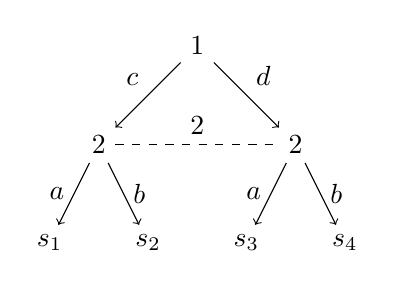
\begin{tikzpicture}[->,level/.style={sibling distance = 2.5cm/#1, level distance = 1.25cm}] ]
\node {1}
    child {
        node (e1) {2}
        child {
            node {$ s_{1} $} edge from parent node [left] {$ a $}
        }
        child {
            node {$ s_{2} $} edge from parent node [right] {$ b $}
        }
        edge from parent node [above left] {$ c $}
    }
    child {
        node (e2) {2}
        child {
            node {$ s_{3} $} edge from parent node [left] {$ a $}
        }
        child {
            node {$ s_{4} $} edge from parent node [right] {$ b $}
        }
        edge from parent node [above right] {$ d $}
    };
\path (e1) edge [-, dashed] node [above] {2} (e2);
\end{tikzpicture}
\caption{Game tree of an example game with imperfect information. First,  player $ 1 $ chooses between the moves $ c $ and $ d $. Player 2 cannot distinguish these moves, so she has to blindly choose between her moves $ a $ and $ b $. This figure is inspired by \cite[fig.~2]{benthem2001a}.}
\label{fig:non-determinancy}
\end{figure}

\subsubsection*{Limitations on the possibility relations}

The presented definition of games of imperfect information is rather broad. It allows for many different kinds of uncertainties. It is possible, that player $ i $ does not know, which move the opponent has played. This is the case of \figref{fig:non-determinancy}. However, more exotic kinds of uncertainties are also possible: It is possible that player $ i $ does not know the outcome of a move he just played himself. It is also possible that he does not know, whose turn it is, what his available moves are, or whether the game has ended. It seem natural to impose limitations on the game trees, such that these kinds of uncertainties are impossible.

First, it is natural to assume that the players know the outcomes of the moves they just played. If we assume that every state $ s $ is labeled with a unique atomic proposition $ s' $, then we can enforce this by requiring the following for all states $ s \in S $ and all actions $ a \in A $: $ \turn_{i} \wedge \langle a \rangle s' \rightarrow \langle a \rangle \know_{i} s' $. Note that this does not guarantee that the players know the outcomes of their moves, \emph{before} they play them. This property is captured by $ \turn_{i} \wedge \langle a \rangle s' \rightarrow \know_{i} \langle a \rangle s' $.

Second, it is natural to assume that the players know, who is next to make a move. This can be enforced by demanding $ \turn_{i} \rightarrow \cknow_{I} \turn_{i} $, where $ \cknow $ is the common knowledge operator and $ I $ is the set of players \cite{benthem2001a}.

Next, it seem natural that the players know what moves are currently possible. That is, the same set of moves should be possible from two states, if the player to move cannot tell apart these two states. Formally, we demand $ \turn_{i} \wedge \langle a \rangle \true \rightarrow \know_{i} \langle a \rangle \true $ for all moves $ a \in A $ \cite{benthem2001a}. If we instead want the currently available moves to be common knowledge, we can demand $ \langle a \rangle \true \rightarrow \cknow_{I} \langle a \rangle \true $.

Finally, if all players should be aware that the game has ended and if this should be common knowledge, we can impose the following limitation: $ \leaf \rightarrow \cknow_{I} \leaf $.

{ \color{red} The interchange principle (the beer example?)}


%\begin{itemize} \color{red}
%\item Formal definition of imperfect-information game trees
%\item Strategies in imperfect games (the discussion from V.3). Maybe it is better to describe this after perfect recall.
%\item Short introduction to outcomes and powers in imperfect games (C3 does not hold anymore).
%\item Remarks on the looseness of this definition: "Players need not know what the opponent has played, or what they played themselves, they need not know if it is their turn, or whether the game has ended, etc. One can think up plausible scenarios with all of the pictures shown in Figure 6."
%\item How to restrict the imperfect-information-game-trees model to be more "realistic": Describe the examples from "III.3. Constraints for special axioms".
%\end{itemize}

\subsection{Liar's Dice}

As an example of a game of imperfect information, we now consider the game Liar's Dice. In this game\footnote{A variety of dice games are called Liar's Dice. They all have elements of concealed die rolls and deception. The variant we consider is probably the simplest.}, two players take turns rolling a single die under a cup, privately looking at the result, and then call out an outcome of the die roll. The player may lie about the outcome of the roll. Now, the opponent can accept the call and start a new round by re-rolling the die or she can challenge the call by lifting the cup. If the call was correct, she looses the game and if the call was a lie, she wins the game. In each round, a player must call out a greater outcome than the one called in the previous round.

This can be formalised as follows \cite{ferguson1991}. In round $n$ player $i$ has the turn and rolls the die. She observes the outcome, which is a random integer $X(n)$ taking the values from 1 to 6 with equal probabilities. Then she announces an integer $y(n)$ between $y(n-1)+1$ and 6, both inclusive, with $y(0) = 0$. The next player $j$ then announces whether she doubts or believes the claim. If $y(n)=6$ then she always doubts. If she doubts then $j$ wins if $X(n) < y(n)$ and $i$ wins otherwise. If she believes then round $n+1$ begins and $j$ has the turn.

\subsection{Perfect recall}
Liar's Dice satisfies the property \emph{Perfect Recall}~\cite{benthem2001a} -- the players remember their own previous moves, as well as the uncertainties they had at each stage. This can be shown, by looking at the game tree and verifying that, for any player $i$ and any two states related by the uncertainty relation $\sim_i$, the sequence of moves (made by $i$) leading to each of the two states are the same. 

Note that for this game, \emph{Perfect Recall} has little significance under the assumption that all agents are rational, since the rounds that came before the previous one shouldn't impact the decision for the current round.

{ \color{red} Predictive strategies? Ask Nina\dots }

\subsection{Indistinguishable actions and Product Update}
We already introduced the notion of epistemic indistinguishability between states, modelled by the uncertainty relation $\sim_i$. Now we will see that a natural next step is to add an uncertainty relation between actions to our game models as well. With this expansion of the uncertainty relation we obtain a more general model, as different actions can lead to the same outcomes. An example of indistinguishable actions in Liar's Dice are those performed by Nature, from the perspective of a player that doesn't have the turn. The \emph{Product Update} mechanism is described as~\cite{benthem2001a}:
$$
(x,a)\sim_i(y,b) \leftrightarrow x\sim_i y \mbox{ and } a\sim_i b
$$
where $(x,a)$ and $(y,b)$ are ordered pairs consisting of 1) previous state, and 2) last made action. It can be used iteratively to compute next levels of game trees.



{ \color{red} Something about the three properties/axioms regarding Product Update. }